\documentclass[12pt,border=1pt]{standalone}
\usepackage[utf8]{inputenc}
\usepackage{pgfplots}
\usepackage{siunitx}
\usepackage{xcolor}

\renewcommand*\sfdefault{phv}
\renewcommand{\familydefault}{\sfdefault}

\pgfplotsset{compat=newest, width=5.5cm,
             xtick pos=left, ytick pos=left,
             xtick scale label code/.code={},
             yticklabel style={text width=2em,align=right}}

\newcommand{\col}{black}
\newcommand{\txt}{white}

\begin{document}
  \begin{tikzpicture}
    %% Chromium
    \node [anchor=south west,inner sep=0] (A) at (0,0)  
      {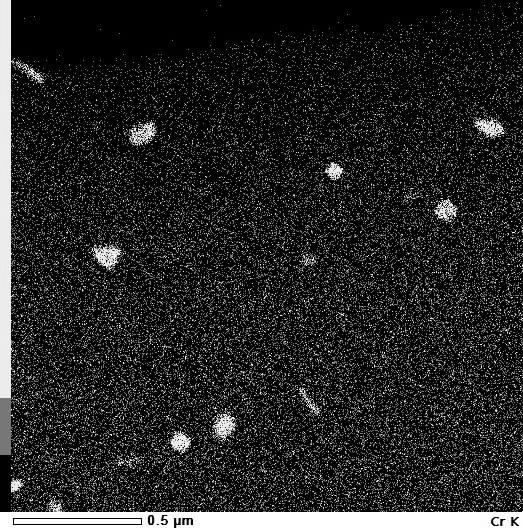
\includegraphics[scale=0.15]{../src/A1/view_003_Cr_K.png}}; 
    \node [right of=A, node distance=3.35cm] (B) 
      {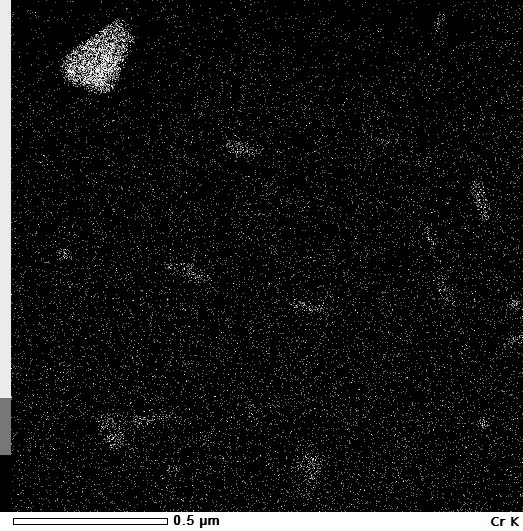
\includegraphics[scale=0.15]{../src/A1/view_004_Cr_K.png}}; 
    \node [right of=B, node distance=3.35cm] (C) 
      {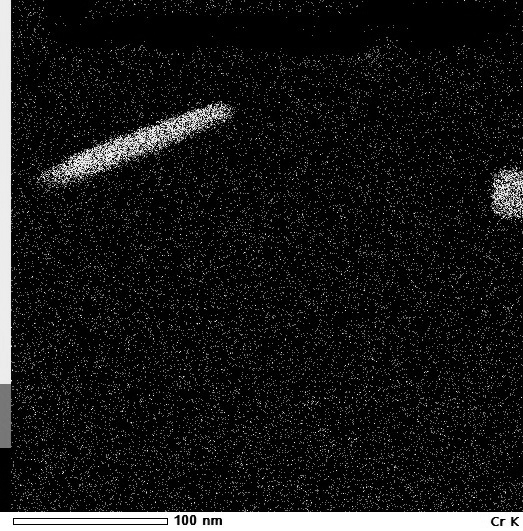
\includegraphics[scale=0.15]{../src/B1/view_000_Cr_K.png}}; 
    \node [right of=C, node distance=3.35cm] (D) 
      {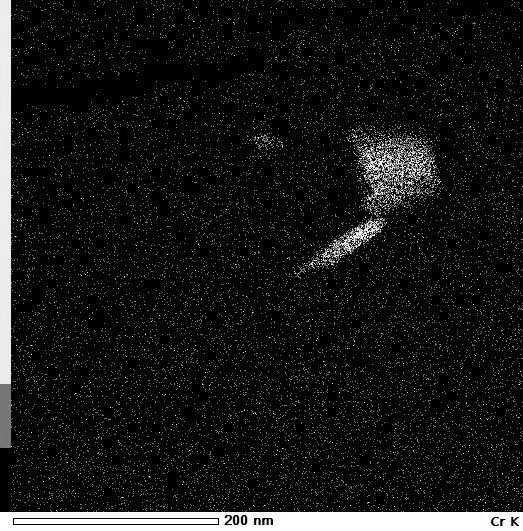
\includegraphics[scale=0.15]{../src/B1/view_001_Cr_K.png}}; 
     %% Nitrogen
    \node [below of=A, node distance=3.35cm] (E) 
      {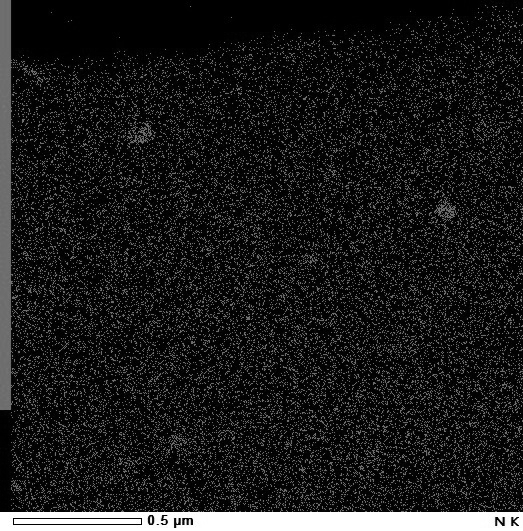
\includegraphics[scale=0.15]{../src/A1/view_003_N_K.png}}; 
    \node [below of=B, node distance=3.35cm] (F) 
      {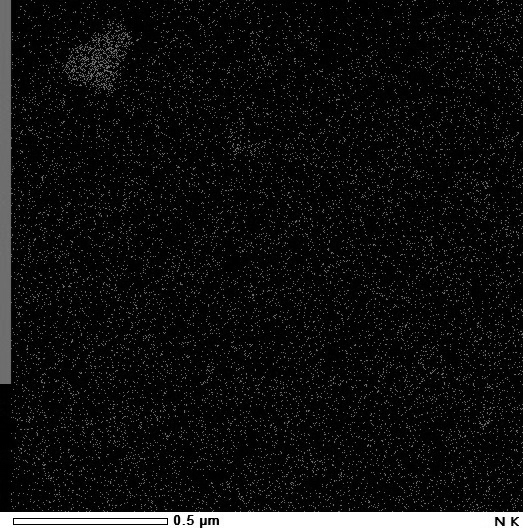
\includegraphics[scale=0.15]{../src/A1/view_004_N_K.png}}; 
    \node [below of=C, node distance=3.35cm] (G)  
      {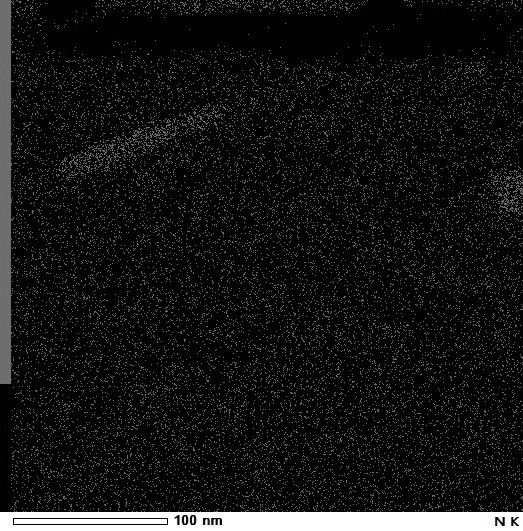
\includegraphics[scale=0.15]{../src/B1/view_000_N_K.png}}; 
    \node [below of=D, node distance=3.35cm] (H) 
      {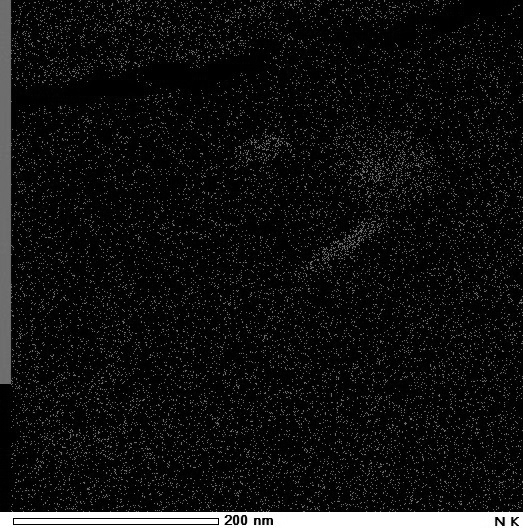
\includegraphics[scale=0.15]{../src/B1/view_001_N_K.png}}; 
    \begin{scope}[x={(A.south east)},y={(A.north west)}]
      %\draw[help lines,xstep=.2,ystep=.2,color=gray] (0,0) grid (2.1,1);
      \filldraw[fill=white,draw=black] 
        (0.00,+0.797) rectangle +(0.2,0.2) node[pos=.5] {\footnotesize Cr};
      \filldraw[fill=white,draw=black] 
        (0.00,-0.390) rectangle +(0.2,0.2) node[pos=.5] {\footnotesize N};
      %% Bars for Cr
      \filldraw[\col,very thick] 
        (0.025,0.02) -- node[above] {\color{\txt}\tiny\SI{0.5}{\micro\metre}} +(0.25,0.0);
      \filldraw[\col,very thick] 
        (1.230,0.02) -- node[above] {\color{\txt}\tiny\SI{0.5}{\micro\metre}} +(0.30,0.0);
      \filldraw[\col,very thick] 
        (2.440,0.02) -- node[above] {\color{\txt}\tiny\SI{100}{\nano\metre}} +(0.30,0.0);
      \filldraw[\col,very thick] 
        (3.640,0.02) -- node[above] {\color{\txt}\tiny\SI{200}{\nano\metre}} +(0.40,0.0);
      %% Bars for N
      \filldraw[\col,very thick] 
        (0.025,-1.165) -- node[above] {\color{\txt}\tiny\SI{0.5}{\micro\metre}} +(0.25,0.0);
      \filldraw[\col,very thick] 
        (1.230,-1.165) -- node[above] {\color{\txt}\tiny\SI{0.5}{\micro\metre}} +(0.30,0.0);
      \filldraw[\col,very thick] 
        (2.440,-1.165) -- node[above] {\color{\txt}\tiny\SI{100}{\nano\metre}} +(0.30,0.0);
      \filldraw[\col,very thick] 
        (3.640,-1.165) -- node[above] {\color{\txt}\tiny\SI{200}{\nano\metre}} +(0.40,0.0);
    \end{scope}
  \end{tikzpicture}
\end{document}